\documentclass[conference]{IEEEtran}
\IEEEoverridecommandlockouts

\usepackage{cite}
\usepackage{amsmath,amssymb,amsfonts}
\usepackage{algorithmic}
\usepackage{graphicx}
\usepackage{textcomp}
\usepackage{xcolor}
\usepackage{caption}
\usepackage{float}
%\usepackage{placeins} % removed to avoid FloatBarrier white-space gaps
\def\BibTeX{{\rm B\kern-.05em{\sc i\kern-.025em b}\kern-.08em
    T\kern-.1667em\lower.7ex\hbox{E}\kern-.125emX}}

\newcommand{\cmark}[1]{\raisebox{.5pt}{\textcircled{\raisebox{-.9pt}{\scriptsize\bfseries #1}}}}

\begin{document}

\title{Active Digital Twin Verification for Robust Federated Learning in IoT Intrusion Detection}

\author{
\IEEEauthorblockN{Hoang-Hao Pham\IEEEauthorrefmark{1}\IEEEauthorrefmark{2}, Phan The Duy \IEEEauthorrefmark{1}\IEEEauthorrefmark{2}, Van-Hau Pham\IEEEauthorrefmark{1}\IEEEauthorrefmark{2}}
\\
\IEEEauthorblockA{\IEEEauthorrefmark{1}Information Security Laboratory, University of Information Technology, Ho Chi Minh City, Vietnam\\}
\IEEEauthorrefmark{2}Vietnam National University, Ho Chi Minh City, Vietnam\\

haoph.16@grad.uit.edu.vn, \{duypt, haupv\}@uit.edu.vn}


\maketitle

\begin{abstract}
Federated Learning has become a practical approach for training intrusion detection models across distributed Internet of Things devices, but it remains exposed to poisoning attacks, non-IID data heterogeneity, and free-rider exploitation. This paper presents DT-Guard, a defense framework that leverages a server-side Digital Twin as a controlled testing environment for actively verifying client model behavior. Each submitted update is deployed in the Digital Twin and evaluated on synthetic challenge data through a four-layer pipeline that examines detection capability, backdoor resistance, parameter deviation, and cross-round stability. A complementary aggregation scheme called DT-Driven Performance Weighting compares client predictions against the current global model, exposing free-riders whose outputs are nearly indistinguishable from the global baseline. We validate DT-Guard on CIC-IoT-2023 under five poisoning strategies. DT-Guard generally outperforms nine existing defenses in accuracy, false positive rate, and contribution fairness.
\end{abstract}

\begin{IEEEkeywords}
Federated learning, Digital twin, Intrusion detection, IoT security, Poisoning attack, Contribution evaluation
\end{IEEEkeywords}

\section{Introduction}

Federated Learning (FL) allows Internet of Things (IoT) devices to collaboratively train shared models, including Intrusion Detection Systems (IDS), while keeping raw data on-device~\cite{mcmahan2016communication}. This privacy-preserving property is attractive for IoT deployments where transmitting full traffic captures to a central server is neither feasible nor desirable. In practice, however, the data residing on individual IoT nodes tends to be non-independent and non-identically distributed (non-IID) with heavy class imbalance, which already complicates the learning process. This heterogeneity also enables sophisticated poisoning and backdoor attacks~\cite{baruch2019little, shejwalkar2021manipulating} that exploit the statistical noise inherent in non-IID settings.

Recent work has attempted to harden FL aggregation against such threats. A comprehensive evaluation in DT-BFL~\cite{issa2025dtbfl} and related studies~\cite{zeng2024clipcluster, xu2022signguard} found that most existing defenses fail against at least one attack type when tested on realistic datasets.

\begin{enumerate}
    \item \textbf{Circumventable defenses.} Modern poisoning attacks, including LIE~\cite{baruch2019little}, Min-Max/Min-Sum~\cite{shejwalkar2021manipulating}, MPAF~\cite{cao2022mpaf}, and Backdoor, have been specifically crafted to evade existing filters. A cross-method evaluation in DT-BFL~\cite{issa2025dtbfl} shows that each defense, whether Krum~\cite{blanchard2017machine}, Median/Trimmed Mean~\cite{yin2018byzantine}, GeoMed~\cite{pillutla2022robust}, SignGuard~\cite{xu2022signguard}, ClipCluster~\cite{zeng2024clipcluster}, or LUP, fails against at least one attack type when tested on the same realistic dataset.

    \item \textbf{Non-IID confusion.} Passive parameter analysis confuses natural Non-IID deviations with intentional manipulation. SignGuard~\cite{xu2022signguard} relies on gradient-sign direction, ClipCluster~\cite{zeng2024clipcluster} on norm clipping and clustering, and LUP~\cite{issa2025dtbfl} on MAD-based outlier removal and parameter distance. These criteria make the systems prone to high false positive rates or to missing attacks that have been reverse-optimized, such as LIE~\cite{baruch2019little} and Min-Max/Min-Sum~\cite{shejwalkar2021manipulating}.

    \item \textbf{Missing contribution assessment.} No existing mechanism quantifies the actual knowledge contribution of each client. FedAvg~\cite{mcmahan2016communication} assigns weights by sample count without reflecting update quality. Trust Score in LUP~\cite{issa2025dtbfl} and PoC in PPSG~\cite{zhang2025ppsg} both measure parameter deviation from the global model, which inadvertently rewards free-riders whose updates are nearly identical to the global parameters.
\end{enumerate}

We introduce DT-Guard to address these gaps. The server maintains a Digital Twin (DT) where each client update is deployed and evaluated on synthetic challenge data. A four-layer verification pipeline produces a Trust-Score that determines acceptance. A separate \textbf{DT-Driven Performance Weighting (DT-PW)} mechanism compares each client's predictions against the global model's predictions on the same data. Clients that have genuinely learned from local data will disagree with the global model in informative ways; free-riders will produce near-identical outputs and are caught by an automatic \emph{Effort Gate}.

Our contributions are as follows. We characterize how adaptive attacks, non-IID confusion, and the free-rider problem jointly undermine existing FL defenses. We then propose DT-Guard, which uses a server-side Digital Twin for behavioral testing instead of parameter inspection. Within this framework we design DT-PW, an aggregation mechanism that scores contributions by inference divergence and filters free-riders through an automatic Effort Gate. Finally, we evaluate DT-Guard on CIC-IoT-2023 under five attack strategies against nine baselines.


\section{Related Works}


\subsection{Background}

A \emph{Digital Twin} (DT) is a live software replica of a physical system that stays in sync with the real counterpart~\cite{issa2025dtbfl}. In our setting the DT runs on the FL server and acts as a sandbox: each client update is loaded into it, tested on challenge data, and scored before the server decides whether to include it in the next global model.

Modern \emph{poisoning attacks} work at either the data or the model level, but the most dangerous variants blend their malicious changes into the normal update distribution so that parameter-level filters miss them. A separate threat is the \emph{free-rider}: a client that simply copies the global model back, contributing nothing new while still receiving the aggregated result. Because its update sits very close to the global parameters, distance-based defenses have no reliable way to flag it.

\subsection{Robust Aggregation Against Poisoning}

Classical robust aggregation rules such as Krum~\cite{blanchard2017machine}, coordinate-wise Median, Trimmed Mean~\cite{yin2018byzantine}, and GeoMed~\cite{pillutla2022robust} filter outliers in parameter space using geometric or order-statistic criteria. While they were effective against first-generation attacks, modern adversaries have learned to stay within the ``safe'' region. SignGuard~\cite{xu2022signguard} introduced gradient-sign analysis to catch directional anomalies, but LIE~\cite{baruch2019little} and Min-Max/Min-Sum~\cite{shejwalkar2021manipulating} explicitly optimize their perturbations to preserve sign consistency. ClipCluster~\cite{zeng2024clipcluster} clips norms and then clusters updates, yet it struggles when malicious updates are placed near the centroid of benign clusters. The most sophisticated approach to date, LUP~\cite{issa2025dtbfl}, combines MAD-based outlier removal with agglomerative hierarchical clustering and a Trust Score derived from parameter deviation. Even so, its Trust Score mechanism inadvertently favors free-riders, whose updates sit closest to the global model.

All these methods rely on parameter-space analysis. Under strong non-IID conditions, benign updates can naturally vary as much as attack-induced perturbations. This leads to false positives or missed detections. DT-Guard uses behavioral testing: each update is exercised on challenge data in the Digital Twin.

\subsection{Digital Twin in FL and IoT}

Several systems have incorporated Digital Twins into FL workflows. DT-BFL~\cite{issa2025dtbfl} builds edge-level DTs that mirror device states and facilitate blockchain interactions. BAFL-DT~\cite{qu2021bafldt} uses a cloud-based DT for model replication and storage. Zhang et al.~\cite{zhang2025ppsg} integrate DT with asynchronous FL in the PPSG framework, where contribution assessment uses Maximum Mean Discrepancy (MMD) between local and global models. Lu et al.~\cite{lu2020diten} deploy DTs at the edge for model training and aggregation (DITEN).

These systems use the DT for infrastructure or resource management. None of them use the DT as a behavioral testing environment where each client model runs on controlled challenge data before acceptance.

\subsection{Contribution Evaluation}

FedAvg~\cite{mcmahan2016communication} weights clients by sample count. This approach ignores update quality. Trust Score in LUP and PoC in PPSG both use parameter distance, which rewards free-riders. Shapley value~\cite{shapley1953value} has been applied to blockchain-FL~\cite{zhang2025bcsm} (HSDPS). Computing exact Shapley values has exponential complexity. Approximations introduce noise. The scores influence consensus selection rather than aggregation weights. None of these methods measure actual inference performance on a representative test set to our knowledge.


In summary, Table~\ref{tab:related_comparison} positions DT-Guard relative to the works discussed above. Its distinguishing features are active behavioral verification, challenge data generated by deep generative models, and inference-based contribution scoring.

\begin{table}[!t]
\caption{Positioning of DT-Guard among Related Works}
\label{tab:related_comparison}
\begin{center}
\footnotesize
\begin{tabular}{|l|c|c|c|c|}
\hline
\textbf{Framework} & \textbf{Year} & \textbf{Verif.} & \textbf{DT Role} & \textbf{Contrib.} \\
\hline
FedAvg~\cite{mcmahan2016communication} & 2017 & None & None & Sample \\
Krum~\cite{blanchard2017machine} & 2017 & Passive & None & Select 1 \\
GeoMed~\cite{pillutla2022robust} & 2022 & Passive & None & None \\
SignGuard~\cite{xu2022signguard} & 2022 & Passive & None & None \\
ClipCluster~\cite{zeng2024clipcluster} & 2024 & Passive & None & Cluster \\
\hline
LUP~\cite{issa2025dtbfl} & 2025 & Passive & Infra. & Trust \\
PPSG~\cite{zhang2025ppsg} & 2025 & Passive & Comp. & PoC \\
HSDPS~\cite{zhang2025bcsm} & 2025 & Passive & None & Shapley \\
\hline
\textbf{DT-Guard} & \textbf{2026} & \textbf{Active} & \textbf{Test} & \textbf{DT-PW} \\
\hline
\end{tabular}
\end{center}
\end{table}

\section{Proposed Method}

\subsection{System Architecture}

DT-Guard aims to produce a robust global intrusion detection model that accurately classifies IoT network traffic, covering both benign flows and multiple attack categories, even when a significant fraction of participating clients submit poisoned or free-rider updates. As shown in Fig.~\ref{fig:framework}, the system involves three entities (IoT Clients, an FL Server, and a server-side Digital Twin Verification Environment) connected by five steps per round:

\begin{enumerate}
    \item[\cmark{1}] \textbf{Upload.} Each client trains its local IDS model on the network traffic it observes and uploads the updated parameters~$\mathbf{w}_i^{(t)}$ to the FL Server.
    \item[\cmark{2}] \textbf{Deploy.} Rather than aggregating immediately, the server deploys every received update into the DT Sandbox. A Challenge Generator (TabDDPM) supplies synthetic traffic samples~$\mathcal{D}_{\text{ch}}$ covering both benign and attack classes (e.g., DDoS, brute force, spoofing). Inside the sandbox, two modules run in parallel: a \emph{Four-Layer Verification Pipeline} that examines detection quality, backdoor resistance, parameter integrity, and cross-round stability to produce a Trust-Score~$T_i$; and a \emph{DT-PW Scoring} module that computes prediction divergence~$d_i$ between the client model and the current global model~$\mathbf{w}^{(t-1)}$.
    \item[\cmark{3}] \textbf{Gate \& Aggregate.} Both scores feed into a decision gate. Updates that fail the trust or effort threshold are rejected; those that pass proceed to DT-PW Aggregation, which merges accepted updates using contribution-based weights.
    \item[\cmark{4}] \textbf{Update.} The newly aggregated global model~$\mathbf{w}^{(t)}$ is returned to the FL Server.
    \item[\cmark{5}] \textbf{Broadcast.} The server distributes~$\mathbf{w}^{(t)}$ back to all clients for local intrusion detection and further training.
\end{enumerate}

  Deploying client models into a separate Digital Twin, rather than running them directly on the FL server, provides two critical benefits. First, it isolates potential malicious behavior: a
  client model with harmful code cannot compromise the server's coordination logic when execution is confined to a sandboxed environment. Second, it allows verification to scale independently: the
  server can spawn multiple DT instances for parallel testing without affecting aggregation or broadcasting, which keeps the main thread responsive even under heavy load.
\begin{figure}[t]
\centerline{
\includegraphics[width=\columnwidth]{dtguard-architecture.pdf}}
\caption{Overview of the DT-Guard architecture.}
\label{fig:framework}
\end{figure}


\subsection{Challenge Data Generation}

Since the FL server has no access to raw client data, it relies on a synthetic generator to produce realistic IoT traffic for the DT. We compare five candidates from two families: \emph{diffusion-based}, including TabDDPM~\cite{kotelnikov2023tabddpm} (MLP denoising), TabSyn~\cite{zhang2024tabsyn} (VAE + latent diffusion), and ForestDiffusion~\cite{jolicoeurmartineau2024forest} (XGBoost denoising, CPU-only); and \emph{GAN-based}, including CTGAN~\cite{xu2019modeling} (conditional tabular GAN) and WGAN-GP~\cite{gulrajani2017improved} (gradient-penalty GAN). All five are benchmarked on CIC-IoT-2023 across four criterion groups: fidelity, coverage \& diversity, conditional control, and efficiency (Fig.~\ref{fig:generator}).

\begin{figure}[t]
\centerline{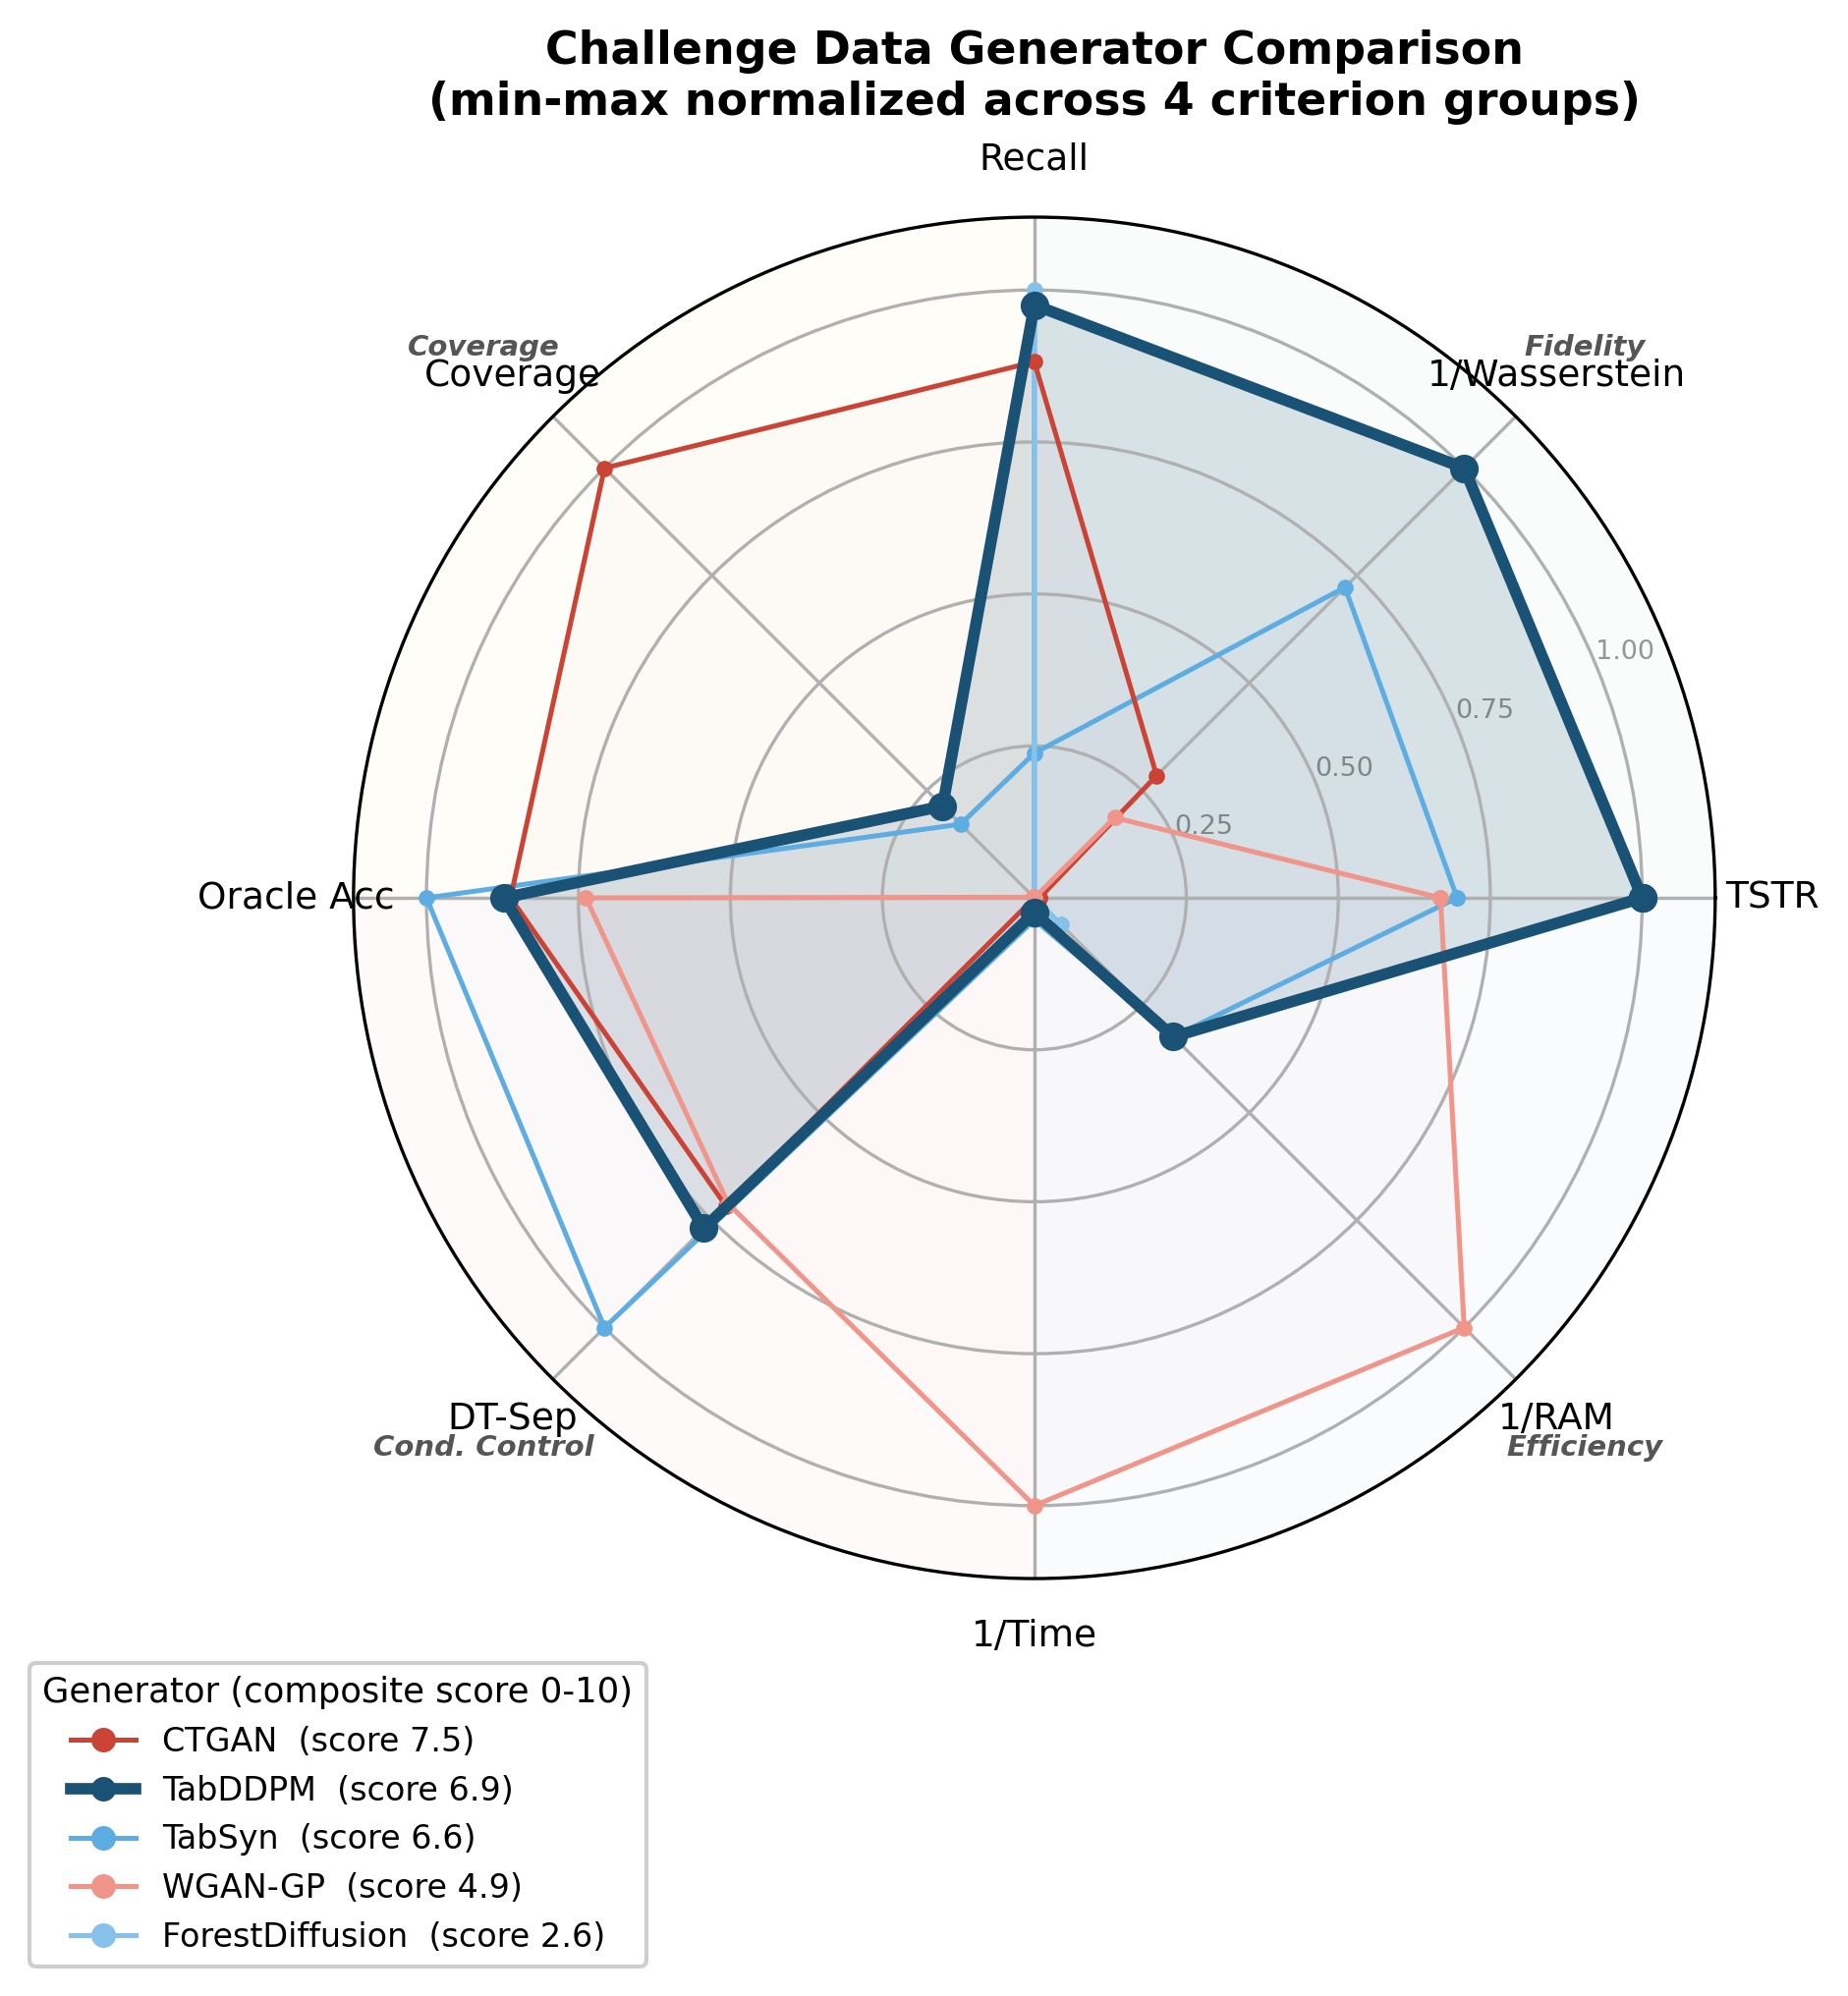
\includegraphics[width=\columnwidth]{fig2_generator_selection.png}}
\caption{A/B testing of five challenge data generators across four criterion groups.}
\label{fig:generator}
\end{figure}

TabDDPM achieves the highest composite score (7.3/10, Fig.~\ref{fig:generator}): it leads in fidelity (TSTR 71.4\%) and diversity (Recall 0.98) while consuming only 200\,s and 25\,MB, over $8{\times}$ faster than CTGAN. TabSyn offers the strongest conditional control but lower recall. CTGAN scores well on coverage yet is too slow for per-round use. ForestDiffusion cannot produce class-conditional samples, and WGAN-GP generates the least diverse data. We therefore adopt TabDDPM as the default challenge generator.


\subsection{Four-Layer Behavioral Verification}\label{sec:fourlayer}

Every candidate update~$\mathbf{w}_i^{(t)}$ is loaded into the DT and evaluated on~$\mathcal{D}_{\text{ch}}$ through four complementary checks. The mechanism is controlled by hyperparameters: $\alpha \in [0,1]$ balances performance vs.\ parameter similarity; $\lambda_{\text{bd}}, \lambda_{\text{stab}} \in \mathbb{R}^+$ are penalty coefficients; $D_{\max} > 0$ normalizes parameter distance; and $\theta_{\text{div}} > 0$ is the divergence threshold for strict mode.

\paragraph{Layer~1: IDS Performance} The model is evaluated on the challenge set using binary classification (benign vs.\ attack). The F1-score serves as the primary quality signal:
\begin{equation}
    s_i^{\text{ids}} = \text{F1}\bigl(\mathbf{w}_i^{(t)},\; \mathcal{D}_{\text{ch}}\bigr) \in [0,1].
\label{eq:ids}
\end{equation}

\paragraph{Layer~2: Backdoor Resistance} Rather than measuring ASR directly (which requires known trigger labels), the DT monitors the variance of prediction confidence across the challenge set. A clean model produces stable confidence; a backdoor-infected model shows abnormally high variance when triggered samples are present. The penalty is:
\begin{equation}
    \delta_i^{\text{bd}} =
    \begin{cases}
        \lambda_{\text{bd}}, & \text{if } \sigma\bigl(\text{conf}(\mathbf{w}_i^{(t)}, \mathcal{D}_{\text{ch}})\bigr) > \tau_{\text{bd}}, \\
        0, & \text{otherwise},
    \end{cases}
\label{eq:bd}
\end{equation}
where $\sigma(\cdot)$ is the standard deviation of the model's softmax confidence on~$\mathcal{D}_{\text{ch}}$ and $\tau_{\text{bd}}$ is the confidence variance threshold.

\paragraph{Layer~3: Parameter Deviation} We compute the mean per-layer $\ell_2$ distance between the client update and the global model, normalized by~$D_{\max}$:
\begin{equation}
    \Delta_i^{(t)} = \frac{1}{L}\sum_{\ell=1}^{L}\frac{\|\mathbf{w}_{i,\ell}^{(t)} - \mathbf{w}_{\ell}^{(t-1)}\|_2}{D_{\max}} \ge 0,
\label{eq:param-dist}
\end{equation}
where $L$ is the number of trainable layers. This is mapped to a similarity score:
\begin{equation}
    s_i^{\text{param}} = 1 - \min\bigl(1,\; \Delta_i^{(t)}\bigr) \in [0,1].
\label{eq:param}
\end{equation}
When $\Delta_i^{(t)} > 1$, the parameters diverge beyond the normalization limit, forcing $s_i^{\text{param}} = 0$.

\paragraph{Layer~4: Cross-Round Stability} Erratic behavior over time is a warning sign. The DT tracks each client's false positive rate over a sliding window of~$\tau$ recent rounds. If the variance exceeds a threshold, a penalty is applied:
\begin{equation}
    \delta_i^{\text{stab}} =
    \begin{cases}
        \lambda_{\text{stab}}, & \text{if } \mathrm{Var}\!\bigl(\text{FPR}_i^{(t{-}\tau)},\, \dots,\, \text{FPR}_i^{(t)}\bigr) > \tau_{\text{stab}}, \\
        0, & \text{otherwise},
    \end{cases}
\label{eq:stab}
\end{equation}
where $\tau_{\text{stab}}$ is the FPR variance threshold.

\paragraph{Trust-Score Fusion} The four layers are combined into a single Trust-Score using an adaptive aggregation function that depends on parameter divergence severity:
\begin{equation}
    T_i = f(s_i^{\text{ids}}, s_i^{\text{param}}; \Delta_i^{(t)}) - \delta_i^{\text{bd}} - \delta_i^{\text{stab}},
\label{eq:trust}
\end{equation}
where the base score aggregation function~$f(\cdot)$ adapts to divergence level:
\begin{equation}
    f(\cdot) =
    \begin{cases}
        \alpha s_i^{\text{ids}} + (1{-}\alpha) s_i^{\text{param}}, & \Delta_i^{(t)} \le \theta_{\text{div}}, \\[4pt]
        \min(s_i^{\text{ids}}, s_i^{\text{param}}), & \Delta_i^{(t)} > \theta_{\text{div}}.
    \end{cases}
\label{eq:trust-aggregation}
\end{equation}
In balanced mode (first case), Layers~1 and~3 contribute proportionally to~$\alpha$, favoring IDS performance. In strict mode (second case), both layers must score high—requiring strong IDS performance \emph{and} low parameter deviation. A client is accepted only when $T_i \ge \theta_T$, where $\theta_T$ is the trust threshold.



\subsection{DT-Driven Performance Weighting}\label{sec:dtpw}

Once a client passes the trust gate, DT-PW quantifies its contribution by comparing its predictions to those of the current global model on the same challenge data.

\textbf{Prediction divergence.} Both~$\mathbf{w}_i^{(t)}$ and~$\mathbf{w}^{(t-1)}$ are loaded into the DT. Their prediction vectors on~$\mathcal{D}_{\text{ch}}$ are compared:
\begin{equation}
    d_i = \frac{1}{M}\sum_{j=1}^{M} \mathbb{1}\!\bigl[\hat{y}_{i,j} \neq \hat{y}_{g,j}\bigr].
\label{eq:divergence}
\end{equation}

\textbf{Effort Gate.} Free-riders contribute nothing. We set an adaptive threshold to flag such behavior:
\begin{equation}
    \theta_E = \mu_d - \beta \cdot \sigma_d,
\label{eq:effort}
\end{equation}
where $\mu_d$ and $\sigma_d$ are the mean and standard deviation of~$\{d_i\}$ across accepted clients. The parameter $\beta$ controls sensitivity. If $d_i < \theta_E$, the client's contribution weight is zeroed out.

\textbf{Performance-Score and final aggregation.} For clients that pass the Effort Gate ($d_i \ge \theta_E$), we combine detection capability with contribution novelty:
\begin{equation}
    P_i = s_i^{\text{ids}} \cdot \frac{d_i}{\max_k\, d_k}.
\label{eq:performance}
\end{equation}
The aggregation weight merges Trust-Score and Performance-Score:
\begin{equation}
    w_i = \frac{T_i \cdot P_i}{\sum_{k \in \mathcal{A}} T_k \cdot P_k},
\label{eq:weight}
\end{equation}
where $\mathcal{A}$ is the set of accepted, non-free-rider clients. The new global model is computed as:
\begin{equation}
    \mathbf{w}^{(t)} = \sum_{i \in \mathcal{A}} w_i \;\mathbf{w}_i^{(t)}.
\label{eq:aggregation}
\end{equation}

\section{Experiments and Evaluation}

\subsection{Environmental Setup}

We use CIC-IoT-2023~\cite{neto2023ciciot}, a real-world IoT traffic dataset with seven attack categories and benign traffic (34 classes, 39 features). The dataset is partitioned across $K{=}20$ clients via Dirichlet-based non-IID sampling ($\alpha{=}0.5$).

The local model, IoTAttackNet, is a fully connected network ($39{\to}256{\to}128{\to}64{\to}34$) with ReLU activation, BatchNorm, and Dropout ($p{=}0.3$). Training uses Adam (lr${=}10^{-3}$), weighted Cross-Entropy, batch size 512, $E{=}3$ local epochs, and $R{=}20$ rounds. For challenge data generation, we compare five candidates: TabDDPM~\cite{kotelnikov2023tabddpm} (256 hidden units, SiLU, $T{=}200$ steps, 100 epochs), TabSyn~\cite{zhang2024tabsyn} (VAE + latent diffusion, 256 hidden units, 100 epochs), ForestDiffusion~\cite{jolicoeurmartineau2024forest} (XGBoost-based, $T{=}200$, CPU-only), CTGAN~\cite{xu2019modeling} (256 hidden units, 300 epochs), and WGAN-GP~\cite{gulrajani2017improved} (256 hidden units, gradient penalty $\lambda{=}10$, 300 epochs). The trust threshold is $\theta_T{=}0.6$.


We evaluate five attacks: Backdoor, LIE~\cite{baruch2019little}, Min-Max, Min-Sum~\cite{shejwalkar2021manipulating}, and MPAF~\cite{cao2022mpaf} at 50\% malicious ratio, against nine baselines: FedAvg~\cite{mcmahan2016communication}, Krum~\cite{blanchard2017machine}, Median, Trimmed Mean~\cite{yin2018byzantine}, GeoMed~\cite{pillutla2022robust}, SignGuard~\cite{xu2022signguard}, ClipCluster~\cite{zeng2024clipcluster}, LUP~\cite{issa2025dtbfl}, and PoC~\cite{zhang2025ppsg}.


\subsection{Defense Robustness}



\begin{figure}[t]
\centerline{
\includegraphics[width=\columnwidth]{fig2_degradation.png}}
\caption{Defense comparison at 50\% malicious clients. (a)~Model accuracy. (b)~Detection rate.}
\label{fig:degradation}
\end{figure}

Fig.~\ref{fig:degradation} reports results at 50\% malicious clients, the hardest ratio we tested. In panel~(a), DT-Guard averages 72.8\% accuracy and stays between 72.5\% and 73.1\% regardless of attack type. LUP is close at 72.2\% overall, though it dips to 70.3\% under Backdoor. SignGuard averages 68.0\% but is less consistent, dropping to 53.7\% under MPAF. The other defenses all have at least one attack that breaks them below 2.3\%: GeoMed under LIE, PoC under LIE and Min-Sum, ClipCluster under MPAF, FedAvg and Krum under Min-Sum and MPAF.

The detection rates in panel~(b) tell a related story. DT-Guard catches 98.3\% of attackers on average---100\% on four of five attacks, 91.5\% on LIE. LUP reaches 97.7\% but misses 11.5\% of Backdoor attackers. SignGuard averages 78.0\%; its weak spot is Backdoor at 45.0\%. ClipCluster and PoC both fall below 50\% on average. FedAvg, Krum, and GeoMed never reject anyone, so their detection rate is 0\%.
Overall, DT-Guard is the only defense that simultaneously maintains the highest accuracy and the highest detection rate across all five attack types, confirming that behavioral verification generalizes where parameter-based filters do not.

\subsection{False Positive Analysis}

Fig.~\ref{fig:fpr} shows how often each defense wrongly rejects honest clients under the same scenario.

\begin{figure}[t]
\centerline{
\includegraphics[width=\columnwidth]{fig3_fpr.png}}
\caption{False positive rate (\%) at 50\% malicious clients.}
\label{fig:fpr}
\end{figure}

DT-Guard maintains 0.0\% FPR across all five attack types---the only active defense to do so while still reaching the highest detection rate (98.3\%, Fig.~\ref{fig:degradation}b). Every other defense that actively rejects clients trades detection for false alarms.

LUP reaches 97.7\% detection but produces 26.7\% average FPR, peaking at 49.5\% under Backdoor: nearly half of honest clients are excluded. PoC is worse, with 74.5\% FPR under LIE and 39.5\% on average. Trimmed Mean averages 25.6\% FPR; GeoMed hits 81.0\% under Min-Sum. ClipCluster keeps FPR at 2.3\% on average, but at the expense of detecting only 47.6\% of attackers.

FedAvg and Krum report 0\% FPR because they never reject any client. Their 0\% detection rate (Fig.~\ref{fig:degradation}b) confirms they simply accept everything, including malicious updates.

The reason DT-Guard escapes this tradeoff is that it judges models by what they \emph{do} on challenge data, not by how their parameters look. A honest client with non-IID data may have unusual parameters, but it still classifies traffic correctly---so the four-layer pipeline lets it pass. Parameter-based filters cannot make this distinction.

\subsection{Contribution Fairness}

We inject 4 free-rider clients (20\%) that copy the global model with negligible noise instead of training. Fig.~\ref{fig:weights} compares four weighting strategies. \textbf{DT-PW} correctly assigns weight~0.0 to all four free-riders and redistributes their share equally among the 16 genuine clients (weight~0.0625 each, i.e., $1/16$), achieving the highest accuracy of 72.97\%.

\textbf{Trust-Score}~\cite{issa2025dtbfl} produces the opposite effect: because it scores clients by parameter proximity to the global model, free-riders (whose updates are nearly identical to the global model) receive a disproportionately high weight of 0.2448, while genuine clients are suppressed to just 0.0013. This weight inversion degrades accuracy to 46.49\%. \textbf{Uniform} and \textbf{FedAvg} assign equal weights (0.05) to all clients regardless of contribution, reaching 72.51\%---comparable to DT-PW only because free-riders echo the global model in this scenario. The Effort Gate (Eq.~\ref{eq:effort}) drives DT-PW's advantage by zeroing clients whose predictions nearly match the global model.
\begin{figure}[t]
\centerline{
\includegraphics[width=\columnwidth]{fig4_weights.png}}
\caption{Per-client aggregation weights averaged over the last 5 of 20 rounds.}
\label{fig:weights}
\end{figure}

\subsection{Computational Overhead}

DT-Guard adds 80.8\,ms per round (less than 1\% of total round time), decomposed into DT verification and DT-PW scoring. This overhead is negligible compared to the multi-minute training rounds typical in IoT FL deployments. Peak memory is 485\,MB, the lowest among all ten strategies, because the sandbox loads one model at a time and frees resources before the next. Source code and reproduction scripts are available at \url{https://github.com/HaoPhamUIT/DT-Guard-FL}.

\section{Conclusion and Future Work}

DT-Guard replaces passive parameter inspection with active behavioral testing in federated learning. By loading client updates into a Digital Twin and evaluating them on synthetic challenge data, the four-layer verification pipeline distinguishes genuine non-IID variation from poisoning based on what models \emph{do} rather than parameter appearance. The DT-PW aggregation mechanism further addresses free-riding by comparing client predictions with the global model and filtering out contributions that add no new knowledge.

Experimental evaluation on CIC-IoT-2023 demonstrates that DT-Guard achieves superior performance compared to nine baseline defenses. The framework maintains high accuracy and detection rates while keeping false positives near zero. Furthermore, DT-PW successfully identifies and suppresses all free-riders, whereas proximity-based aggregation methods inadvertently assign them high weights. The computational overhead remains acceptable for practical deployment.

Future research directions include validating DT-Guard on additional IoT security datasets, developing adaptive threshold mechanisms for dynamic attack scenarios, and extending the framework to asynchronous federated learning environments.


\bibliographystyle{IEEEtran}
\bibliography{references}

\end{document}
